\ \\[-10cm]
The previous part of this guide explored some of the main challenges of communicating multiple computers.
The \concept{Internet} is one working solution to those challenges: the one humans have created over the last half century,
now central to many social, commercial and political activities. 
% 
This part studies the main features offered by the Internet, as well as the \concept{suit} of \conceptRef{protocol}{protocols} 
employed to achieve them.


\chapterimage{earth.jpg}

\chapter{The Internet}\label{sec:internet}

Modern communications are based on layered network \conceptRef{stack}{stacks}. 
Maybe you just downloaded this guide from the Internet.
% 
What layers are used exactly? What protocols are employed, and with what purpose?
% 
This chapter provides a primer to answer these questions.\\[-1cm]

\section{The TCP/IP stack}


The \concept{Internet} is a practical solution to the problem of global computer communication,
whose development started in the late 1960's -- early 1970's, and is still ongoing.

\conceptRef{packet}{Packet} switching was conceived during the early 1960s, and the first 
wide-area implementation, \concept{ARPANET}, began in 1969. 
% 
A key challenge at the time was to interconnect existing \conceptRef{network}{networks}, 
owned by different organizations, and based on different technologies and \conceptRef{protocol}{protocols}.
% 
To make things viable, all the following requirements had to be met:
\begin{itemize}
    \item Existing networks should work without updates to the physical infrastructure 
      or their protocols, just the way those protocols are used.
    \item Existing networks should remain independently managed at the local level (autonomous internal organization).
    \item Packets may not always be delivered, some are lost.
    \item Messages that arrive may not be in order, and may be repeated.
\end{itemize}

The solution adopted by ARPANET --and later by the whole world-- 
is the \concept{TCP/IP} protocol suite, first described in 1974. 
It is a layered approach, designed to be ``plugged-in'' on top of 
existing \conceptRef{LAN}{LANs}, with the goal of offering networking 
capabilities to all user applications.

\begin{center}
\begin{bytefield}{16}
\begin{rightwordgroup}[curlyshrinkage=10pt]{User programs}
\wordbox{3}{Layer 7: Application}
\end{rightwordgroup} \\
\begin{rightwordgroup}[curlystyle=\color{color1},curlyshrinkage=10pt]{{\color{color1} TCP/IP}}
\wordbox{1}{Layer 4: Transport}\\
\wordbox{1}{Layer 3: Internet}
\end{rightwordgroup} \\
\begin{rightwordgroup}[curlyshrinkage=10pt]{Existing/future LAN technologies}
\wordbox{1}{Layer 2: Network}\\
\wordbox{1}{Layer 1: Physical}
\end{rightwordgroup}
\end{bytefield}
\end{center} 
 
In a nutshell, the main services offered by these layers are as follows:
\begin{enumerate}
\item[\textbf{Layer 1}] \textbf{(Physical)}: 
  Send \concept{digital} data through \concept{analog} media.
\item[\textbf{Layer 2}] \textbf{(Network)}:
  Identify and communicate devices within the same \concept{LAN}.\\
  The term ``Data Link'' layer (from the OSI model) is sometimes used.
\item[\textbf{Layer 3}] \textbf{(Internet)}:
  Identify and communicate devices across all \conceptRef{LAN}{LANs}.\\
  The term ``Network'' layer (also from OSI) is sometimes used.
\item[\textbf{Layer 4}] \textbf{(Transport)}:
  Identify and communicate programs (services).\\
  Also (choose \textit{only} one):
  \begin{enumerate}[label=\alph*)]
   \item Make sure a \concept{stream} of data successfully reaches the other end, 
   and in order \\-- \textit{but} an \concept{overhead} is introduced 
   and \conceptRef{connection}{connections} must be established (\concept{TCP}).
     
   \item Use simple, relatively efficient messages, and have a small overhead\\
   -- \textit{but} messages may be lost, reordered or duplicated (\concept{UDP}).
  \end{enumerate}
\item[\textbf{Layer 7}] \textbf{(Application)}:
  Do anything the user might need. \\
  Don't forget about security (\eg, cryptography) 
  or about efficiency (\eg, compression): Layers 4 and below don't provide that.
\end{enumerate}

\section{TCP/IP protocol overview}

Multiple \conceptRef{protocol}{protocols} are defined to implement the functionality
of each \concept{layer}. These definitions include the required \concept{packet format},
the rules to exchange those packets and their semantics.
% 
These protocols must be understood as a system, in which each part has very specific tasks.

Some of the most relevant protocols to communications using the Internet 
are shown in the next figure. In it:
\begin{itemize}
\item Solid arrows indicate a protocol being encapsulated in another. 
  If the destination is a layer, one protocol within that layer must be used.

\item Dashed boxes indicate auxiliary protocols defined to help other function. 
Dashed arrows indicate what layer uses what auxiliary protocol.

\item Boxes with thicker lines indicate the protocols highlighted in this guide.
\end{itemize}

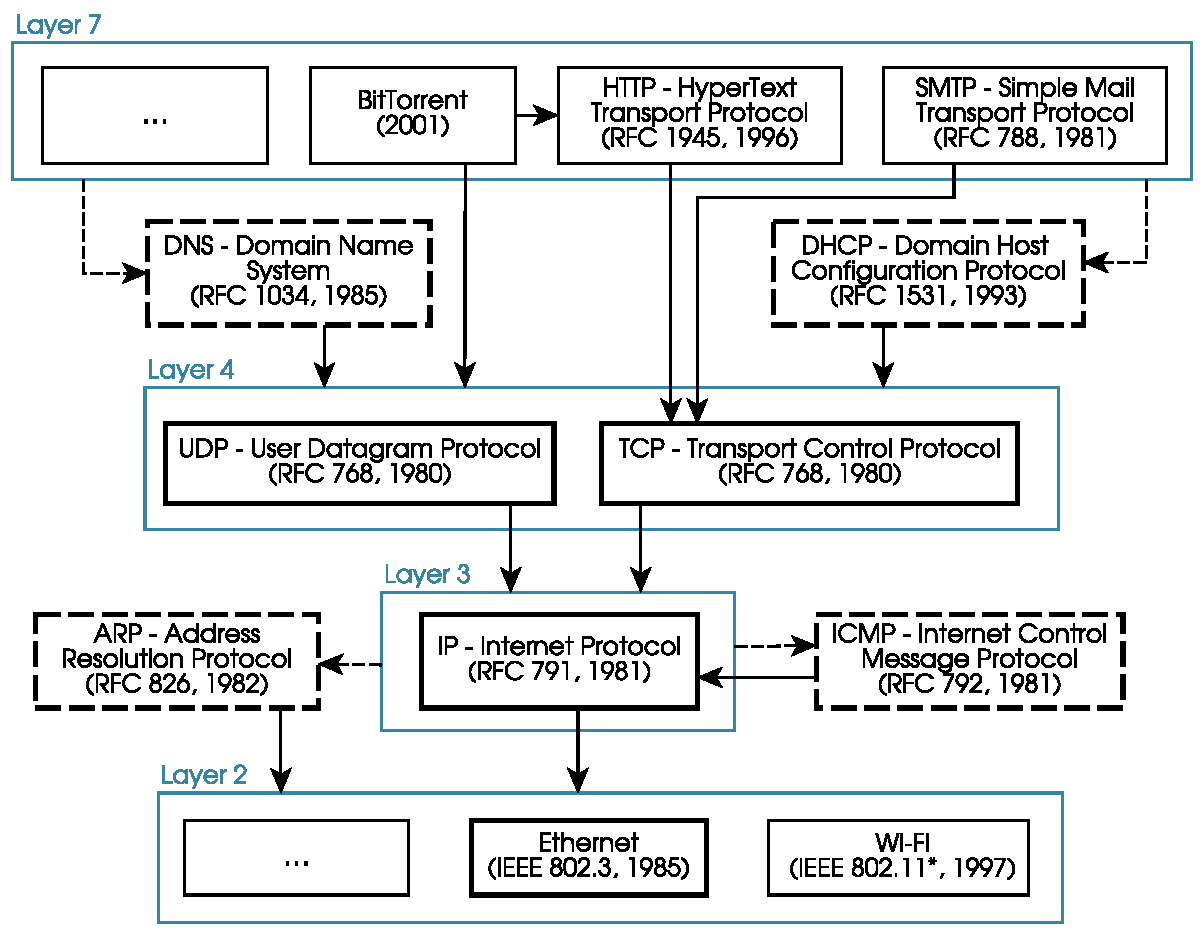
\includegraphics[width=\linewidth]{protocol_dependencies.pdf}

\begin{exercise}
We want to send the sentence ``Sorry, I'll be 5 minutes late'' by email.
Our email client will send those data using the SMTP protocol, which in turn
uses TCP (part of Layer 4).
% 
Assuming SMTP uses headers in its \concept{PDU}, how many headers will 
the corresponding Layer-2 \concept{PDU} contain?
\end{exercise}

\begin{exercise}
Why do you think Layer~3 has only one protocol (two if you count IPv4 and IPv6 separately)? 
\end{exercise}

\section{Who is the Internet boss?}

The \conceptRef{IETF}{Internet Engineering Task Force (IETF)} was created in 1986
to develop and publish standards to be used in the Internet. 
% 
Their main output are  \conceptRef{RFC}{``Request for Comment'' (RFC)} documents,
which contain complete technical descriptions of those standards.


These RFCs are created by working groups of experts, 
for everyone to use freely and free of charge. 
% 
Anyone can participate in these working groups, including researchers,
governments and industry stakeholders. 
% 
Decisions are made when 80-90\% of the participants agree, so no single 
entity controls the standardization process.
% 
\begin{remark}
``We reject kings, presidents, and voting. 
We believe in rough consensus and running code'' 
--- Dave Clark (IETF), 1992.

See DOI \href{https://dx.doi.org/10.1109/MAHC.2006.42}{\underline{10.1109/MAHC.2006.42}} for 
a short story of struggle for power.
\end{remark}

RFCs standards are descriptive, not prescriptive. This means that nobody polices the correct 
use of these standards. Instead, manufacturers have the incentive to be compliant with the RFCs 
so that their products are compatible with others. 
% 
The value of RFCs (and any other standard) is dependent on whether
they are adopted by users. RFCs can be updated and \conceptRef{retire (standard)}{retired} for this reason.

TCP/IP protocols prevail because they are flexible and work reasonably well in most situations, 
even though they are not optimal in virtually any of them. 
Also, TCP/IP protocols are free, as opposed to \concept{privative} protocols
that forced the purchase of a specific vendor's solution.
% 
\begin{remark}
Today it is hard to imagine a world \textit{not} 
dominated by the TCP/IP architecture, 
but entirely different stacks were commercialized and supported until the late 90s.
Examples include AppleTalk and IPX/SPX, by Apple and Novell, respectively.
\end{remark}

% https://www.icann.org/en/blogs/details/cheers-to-the-multistakeholder-community-30-9-2016-en

Some aspects of TCP/IP like unique identifiers 
(including \concept{DNS}, the Domain Name System)
and reserved numbers need to be agreed upon by everyone for the Internet to work properly.
% 
The \concept{IANA} (Internet Assigned Numbers Authority) works in coordination with the \concept{IETF}
to define the appropriate \conceptRef{RFC}{RFCs}.

\begin{remark}
Since 2016, IANA is managed by a nonprofit multistakeholder organization 
(\conceptRef{ICANN}{ICANN - Internet Corporation for Assigned Names and Numbers}).
% 
Since 2004, the responsibility for regional domains 
(\eg, \url{.cat}, \url{.fr}, \url{.es}) is transferred to continent-level 
organizations called regional Internet Registries (\conceptRef{RIR}{RIRs}).
\end{remark}



% # Based on https://www.youtube.com/watch?v=oIezCGjxV3A
% year,text
% 1962,Packet Switching
% 1969,ARPANET
% 1974,TCP/IP
% 1986,IETF
% 1991,WWW
% 1993,CIDR addressing
% 1998,Google
% ``The Internet doesn't do what the endpoints can do (\eg, reliability or compression).''


% - In February 1980, the Institute of Electrical and Electronics Engineers (IEEE) started project 802 to standardize local area networks (LAN).[16][27 (https://en.wikipedia.org/wiki/Ethernet)

% "protocols": "the first sheet of a volume" (on which contents and errata were written

% \begin{remark}
% Extra:
% \begin{itemize}
%     \item Video: https://www.youtube.com/watch?v=oIezCGjxV3A (part 1), https://www.youtube.com/watch?v=RN4gSBTANUY (part 2)
%     \item Monographic: https://cacm.acm.org/research/on-the-hourglass-model/
% \end{itemize}
% \end{remark}


% \begin{itemize}
% \item [\textbf{Layer 1}:] \textbf{Physical}
%     \begin{itemize}
%     \item[Features:] Ship \concept{digital} \otherBase{0}s and \otherBase{1}s through the real, \concept{analog} world.
%     \item[Offers:] Send and receive blocks of bytes.
%     \end{itemize}
% 
% \item [\textbf{Layer 2}:] \textbf{Network}\\
% 
% 
% \item [\textbf{Layer 3}:] \textbf{Internet}\\
% \item [\textbf{Layer 4}:] \textbf{Transport}\\
% \item [\textbf{Layer 7}:] \textbf{Application}\\
% \end{itemize}
% 
% \begin{remark}
% The \concept{OSI} model is a conceptual stack of layers that divides problems a bit differently from \concept{TCP/IP}. 
% TCP/IP was created on the go while the infrastructure of the Internet started its development, became its de-facto standard,
% and is used everywhere. The OSI model is useful to analyze and design communication protocols, but has limited practical usage.
% \end{remark}
% 
% 
% The network stack is normally part of the \concept{operating system} (OS).
% Only the \inlineCode{send} and \inlineCode{receive} functions of Layer 4 are exposed to the users of the OS.
% %
% This way, data transmitted by the \concept{network interface} are guaranteed to be properly formatted and follow
% the protocols of each stack layer.
% 
% \begin{remark}
% In order to control the lower layers --\eg, to transmit custom PDUs--, one needs to be the \texttt{root} user
% or give the \texttt{CAP\_NET\_RAW} kernel capability to a user program
% (or the equivalent in privative systems).
% \end{remark}
% 
% 
% \section{}\label{sec:stack_layers:organization}
% 
% - internet organization 
% bodies and stuff
